\documentclass[sigconf]{acmart}

\AtBeginDocument{%
  \providecommand\BibTeX{{%
    \normalfont B\kern-0.5em{\scshape i\kern-0.25em b}\kern-0.8em\TeX}}}

\usepackage{dblfloatfix}
\usepackage[acronym]{glossaries}

\begin{document}

\newacronym{SMART}{SMART}{SeMantic AnsweR Type}
\newacronym{ATP}{ATP}{Answer Type Prediction}
\newacronym{BERT}{BERT}{Bidirectional Encoder Representations from Transformers}

%\title{Semantic Answer Type Prediction 2020}
\title{%
  Semantic Answer Type Prediction 2020 \\
  \large Team-001}

% AUTHORS:
\author{Stephan Frederik Werner Brandasu}
\affiliation{University of Stavanger}
\email{sf.brandasu@stud.uis.no}

% DATE:
\date{\today}



\begin{abstract}
We describe our solution to the \gls{SMART} prediction task 2020 for the DBpedia dataset. Our methods will take advantage of BM25 scores that get modified by the presence of specific keywords in the questions.
\end{abstract}

\keywords{information retrieval, answer category classification, answer type prediction, natural language understanding, understanding query types}

%% Remove copyright footer
\settopmatter{printacmref=false}
\setcopyright{none}
\renewcommand\footnotetextcopyrightpermission[1]{}
\pagestyle{plain}
%% ------------------------

%%
%% This command processes the author and affiliation and title
%% information and builds the first part of the formatted document.
\maketitle

\section{Introduction}
%Explain the context of the problem that you are tackling, including references to relevant literature.
%% shorten some of the sentences. and maybe increase the introduction length.
%% what are we doing, why is it important and why is it hard.
%% clarify its its question answering or question type answering
\gls{ATP} is a challenging problem in the natural language processing field which is an important step to being able to understand natural language queries. Understand the category and type of a given question is an important step in reaching this goal.

The \gls{SMART} task has provided 2 datasets, one using the DBpedia ontology and another using the Wikidata ontology.
Both datasets follow the same structure and will have a question id, a question text in natural language, an answer category and an answer type. They do differ in one sense though, If the category is a 'resource' then the types from the DBpedia dataset are different from the ones in the Wikidata dataset. This has to be taken into account when attempting to classify the questions.

The goal of this paper is to as accurately as possible classify the category and type of a natural language question.

\section{Related Works}
% add some papers from the smart task, only 2 references so far.
% talk about common methods as well 
% change the heading title
\subsection{Question word categories}
A previous submission to the \gls{SMART} task by \citet{Maryland:qwords} from the University of Maryland found that the category of an answer is highly dependent on the question words. They found for example that questions starting with 'Is' or 'Does' always expect a boolean answer and questions starting with 'when' could expect either a number or a date\cite{Maryland:qwords}. A graph showing the most common question words found by this paper can be seen in figure \ref{figure:firstquestionwords}. 

\begin{figure}[h]
    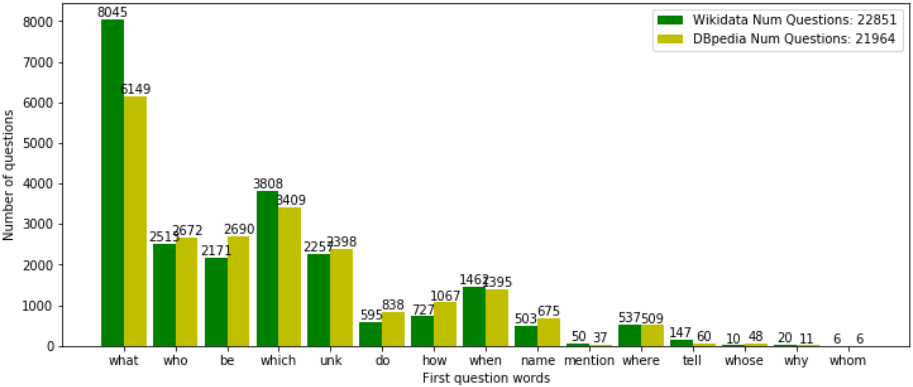
\includegraphics[width=0.45\textwidth]{figures/firstQuestionWords.png}
    \caption{"First words in sentences from Wikidata and DBpedia datasets" by \citet{Maryland:qwords}}
    \label{figure:firstquestionwords}
\end{figure}

\subsection{Most frequent resource types}
The submission by \citet{Kothen:analysis} from the University of Applied Sciences in Kothen Germany did some analysis on the dataset and found that which types of resources came up most commonly over the whole dataset. This information can be used to weigh the possible answers to try to deduce the correct answer type for a given question\cite{Kothen:analysis}. A graph showing the most common answer types found by this paper can be seen in figure \ref{figure:top10resourceanswertypes}.

\begin{figure}[h]
    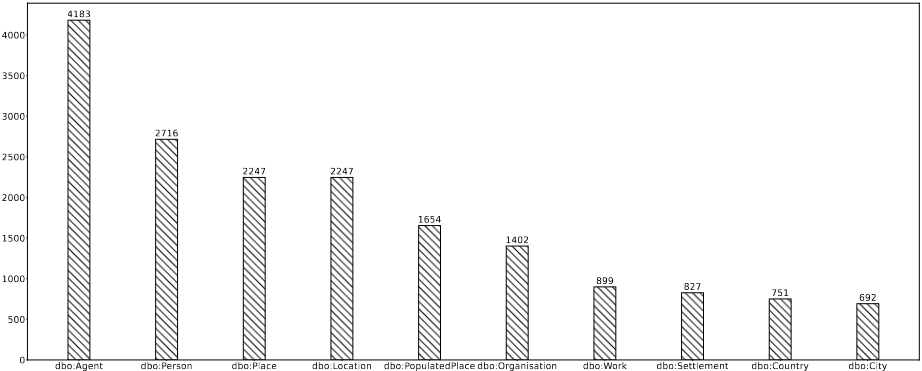
\includegraphics[width=0.45\textwidth]{figures/top10ResourceAnswerTypes.png}
    \caption{"TOP 10 resource answer types" by \citet{Kothen:analysis}}
    \label{figure:top10resourceanswertypes}
\end{figure}

\subsection{Common methods for classification}
A model used frequently used for question classification by previous submissions is \gls{BERT}\cite{maastricht:bert}\cite{heraklion:bert}\cite{tokyo:bert}\cite{uis:bert}\cite{Kothen:analysis}. 

\gls{BERT} is an open source machine learning framework used for natural language processing. The model has been pre-trained but also can be fine-tuned with your own datasets. What is unique about BERT is that it can learn bidirectional representations with transformers. This allows for much larger data sets to be analyzed more quickly since words can be processed in relation to all other words at once, instead of one at the time. Additionally by using transformers \gls{BERT} can better understand the context of a word since it compares it to all the other words at once, this makes it extremely capable for text classification tasks such as this.\cite{nvidia:bert}



%\subsection{DATASETS}
%According to Nahandama Nihindukulasooriya et al rather than building a benchmark from scratch many datasets for semantic answer type prediction are created from existing academic benchmark for base question answering. In creating answer type prediction gold standards they used QALD-9,LC-QuAD v 1.0 and  LC-QuAD v2.0 datasets. The referenced datasets contain natural language query and a corresponding SPARQL query. Gold standard SPARQL query is used to generate results and analyze them to generate an initial answer type for each query and validating them manually.




\section{Problem Statement}
%Formalize the task (in terms of input and output) and specify important details about the data collection.

% problem statement should be a bit longer, talk about datasets that we use. 
% talk about 2 step approach
The objective of this task is to take a natural language question and correctly classify the category and types expected from said question. More broadly this means that a systems needs to be created which takes a normal human written sentence and knows whether to categorise this question as a resource, a literal or as a boolean. Depending on the category it must also identify the correct types for each given category. 

A boolean can only have boolean as a type. Meanwhile a literal could be expecting a string, a date or a number as a type. Resources expect more specific type predictions, first of all if the category is resource then there is a chance more than 1 type is expected as an answer. Second of all the types are expected to exist within a hierarchy based on how specific they are.



%% finish up until here for deadline 1
\section{Baseline Method}
%Explain what you are taking as your baseline method, as well as why this is a reasonable baseline, and why you are making specific implementation choices.
The baseline method used is a basic BM25 implementation from the $rank-bm25$ Python library. The reason for using normal BM25 instead of BM25F or BM25+ is that these modifications aim to improve BM25's performance on multi fielded documents or when dealing with documents with large variance in length but this is not something we need to take into account here.

The input questions and the training data was preprocessed to make it lower case, remove punctuation, stem them and return each question as a list of words. Stopwords are not being removed because questions are so short that the stopwords become a useful part of the context of the question. The results from the preprocessing and the BM25 scoring can be seen in table \ref{tab:baseline_res}

\begin{table}[h]
    \centering
    \caption{Baseline method results}
    \begin{tabular}{c|c|c}
    $Accuracy$ & $NDCG@5$ & $NDCG@10$ \\
    \hline
    0.342 & 0.113 & 0.112
    \end{tabular}
    \label{tab:baseline_res}
\end{table}

In the baseline method the category and type predictions were not done separately. This means that when the program is scoring the question against each question in the training dataset it simply takes the category and types from the highest matched question without any other modifications.

Additionally the scoring is done by multiple parallel processes using the standard multiprocessing library. This allows the algorithm to finish processing the dataset much faster. While this doesn't improve the score this will be useful to more quickly test any changes being made in the advanced method and see if they improve the results as expected.



% finish up until here for deadline 2
\section{Advanced Method}
%Explain what you are taking as your advanced method(s), as well as why this is a promising attempt to outperform the baseline method, and why you are making specific implementation choices.

trying to weigh answer type based on the first word of a question (who, where, what, why) 

\begin{table}[h]
    \centering
    \caption{Advanced method results}
    \begin{tabular}{c|c|c}
    $Accuracy$ & $NDCG@5$ & $NDCG@10$ \\
    \hline
    TODO & TODO & TODO
    \end{tabular}
    \label{tab:baseline_res}
\end{table}


\section{Results}
%With tables and graphs, make a clear, concise, and digestible presentation of the data produced by your experiments. This includes describing the key facts and trend from your results.


\begin{table}[h]
\begin{center}
\caption{Summary of results}
\begin{tabular}{l|c|c|c}
     & $Accuracy$ & $NDCG@5$ & $NDCG@10$ \\
    \hline
    Baseline & 0.342 &  0.113 & 0.112 \\
    Advanced Method & TODO & TODO &  TODO \\
    Advanced Method 1 & \textbf{TODO} & \textbf{TODO} & \textbf{TODO} 
\end{tabular}
\label{table:1}
\end{center}
\end{table}

\section{Discussion and Conclusions}
%Summarize and discuss different challenges you faced and how you solved those. Include interpretations of the key facts and trends you observed and pointed out in the Results section. Which method performed best, and why? Speculate: What could you have done differently, and what consequences would that have had?



%%
%% If your work has an appendix, this is the place to put it.
%\appendix

%\section{Appendix}


%%
%% The next two lines define the bibliography style to be used, and
%% the bibliography file.
\bibliographystyle{ACM-Reference-Format}
\bibliography{base}

\newpage
\appendix
\section{GitHub}
The project code and datasets can be found here:
\href{https://github.com/sbthepotato/DAT640-Project-22H}{github.com/sbthepotato/DAT640-Project-22H}

%\section{Division of Work During the Project}

% remember to keep this up to date
%\begin{center}
%\begin{tabular}{c|c|c|c} 
% week/name & Evans & Peter & Stephan \\ 
% \hline
% 39 & 0 & 0 & 4 \\ 
% 40 & 0 & 0 & 6 \\ 
% 41 & 0 & 0 & 4 \\
% 42 & 0 & 0 & 10 \\
% 43 & 0 & 0 & 12 \\
% 44 & 0 & 0 & 0 \\
% 45 & 0 & 0 & 0 \\
% 46 & 0 & 0 & 0 \\
%\end{tabular}
%\end{center}


\end{document}
\endinput
